\documentclass[journal,11pt,twocolumn]{IEEEtran}
\usepackage[portuguese]{babel}
\usepackage[utf8]{inputenc}
\usepackage[dvips]{graphicx}
\usepackage{amsmath,amsfonts,amssymb}
\usepackage{makecell}
\usepackage[normal]{subfigure}
\usepackage{array,colortbl}
\usepackage{amsmath}
\usepackage{mathrsfs}
\usepackage[sort]{cite}
\usepackage[none]{hyphenat}
\usepackage{minted}
\usepackage{url}
\usepackage[section]{placeins}


% Those packages were originally here, but I don't think we are gonna need them, so I commented them out
%\usepackage[center,small]{caption}
%\usepackage{color}
%\usepackage{colortbl}
%\usepackage{comment}
%\usepackage{float}
%\usepackage{flushend}
%\usepackage[mathfrak]{mathpi}
%\usepackage{morefloats}
%\usepackage{multicol}
%\usepackage{multirow}
%\usepackage{psfrag}
%\usepackage{rangecite}
%\usepackage{tabularx}
%\usepackage{threeparttable}

\graphicspath{ {images/} }
\setminted{breaklines=true}

\sloppy
\newcommand{\goodgap}{%
\hspace{\subfigtopskip}%
\hspace{\subfigbottomskip}}
\newcounter{mytempeqncnt}

\begin{document}

% paper title
\title{Projeto I: Modelos de simulação de canais externos}


\author{Vinícius Dantas de Lima Melo
    \thanks{Este trabalho foi como parte do curso de Comunicações Móveis oferecido pelo Departamento de Engenharia de Comunicações da UFRN.}
}

% The paper headers
\markboth{DCO1020 - Comunicações Móveis}{DCO1020 - Comunicações Móveis}

% make the title area
\maketitle

\begin{abstract}
Esse trabalho realiza discorre a respeito de dois modelos clássicos para simulação de canais externos: o modelo de Clarke/Gans e o modelo de Jakes. A simulação de canais é uma atividade extremamente importante porque torna possível simular soluções e investigar problemas sem precisar de medições, reduzindo custos e aumentando a praticidade.
\end{abstract}

\begin{keywords}
Caracterização de canal, simulação, desvanecimento, sombreamento, outdoors.
\end{keywords}

%\IEEEpeerreviewmaketitle

\section{Introdução}
Simulação do impacto de canais e dos elementos nele presentes é uma tarefa extremamente importante para tornar possível análise de problemas, assim como síntese de novas modelagens e técnicas de transmissão para o dado canal. A possível reproducibilidade fornecida por simulações faz com que se possa analisar e depurar problemas, reduzindo os custos relacionados a suas correções e respectivos testes. 

\subsection{Proposta do Trabalho}
Descrever-se-á e simular-se-á dois diferentes formas de modelar um canal móvel externo. Para as simulações, far-se-á uso de diferentes velocidades relativas para que se possa melhor observar o impacto desse parâmetro em um sistema.

\subsection{Metodologia}
Para as simulações realizadas, foram-se utilizados cálculos feitos em scripts em Python utilizando as bibliotecas Numpy (versão 1.16.2) e Scipy (versão 1.2.1) para computação científica e Matplotlib (versão 3.0.3) para plotagem. Os scripts rodaram sobre o interpretador padrão do Python 3.7.1, sobre o qual foram feitos todos os testes, embora espera-se que ele rode sem problema em interpretadores a partir da versão 3.6, pois faz uso de interpolação literal de strings, adicionada nessa versão a partir da PEP 498~\cite{fstrings}.

Utilizando o submódulo stats da biblioteca Scipy, geraram-se amostras aleatórias a partir de uma variável aleatória que segue a distribuição Gaussiana normal.

Já para transformadas rápidas diretas e inversas de Fourier, utilizou-se o submódulo fft da biblioteca Numpy. Esse submódulo disponibiliza, de maneira imediata, os métodos fft e ifft.

\section{Modelos de canal}
Todas as análise foram feitas utilizando o código disponibilizado junto com o artigo e disponível em um repositório git hospedado do Github, disponível através do link \url{https://github.com/viniciusd/DCO1020---Mobile-Communications/tree/master/assignment1}.

Em \cite{mimo}, vemos que os modelos que aqui serão retratados são baseados em filtragem de ruído branco Gaussiano (FWGN). Esses canais serão caracterizados basicamente pelo espectro Doppler, que governa a variação do tempo no ganho do canal.
\subsection{Modelo de Clarke/Gans}

Adiciona-se, em \cite{mimo}, que o modelo dw Clarke/Gans parte da assunção de que os componentes transmitidos ao redor de uma estação móvel são uniformemente distribuídos e com potências idênticas. Foi-se proposto e aprimorado, respectivamente, por Clarke e Gans em \cite{clarke} e \cite{gans}.

Esse modelo submete duas fontes de ruído gaussianas a filtros de Doppler e, unindo-os, gera a envoltória do canal, que possui o comportamento de uma distribuição de Rayleigh.

Sua implementação foi feita baseada no código descrito no livro, embora com ligeiras adaptações tanto por causa da linguagem escolhida para seu desenvolvimento quanto para reduzir sue consumo de memória.

A partir do código feito, simulou-se o efeito sobre o canal para três diferentes velocidades relativas: 3km/h, 60km/h e 120km/h, conforme visualizado em \ref{gans-3km-h}, \ref{fig:gans-60km-h} e \ref{fig:gans-120km-h}.

Para determinar a frequência de amostragem, uma vez que temos um sinal em banda passante, utilizou-se a inequação exposta em \ref{eq:fs-ineq}. Essa inequação foi exposta em \cite{bandpass}, aonde $f_{U}$ representa a frequência mais alta do sinal e $f_{L}$ sua frequência mais baixa. Para tais frequências, utilizou-se o desvio de frequência de Doppler em relação à frequência central do sinal dado, 1900MHz.
\begin{equation}
    \frac{2f_{U}}{n} \leq f_{s}\leq \frac{2f_{L}}{n-1}
    \label{eq:fs-ineq}
\end{equation}
De forma que se utilizasse um valor de $f_{s}$ que satisfizesse a inequação, optou-se pela expressão \ref{eq:fs-eq}, aonde certamente a média entre os dois extremos satisfazem à ineqaução \ref{eq:fs-ineq}. Isso se dá porque a média entre valores sempre se localiza entre o menor e o maior valor do conjunto.
\begin{equation}
     f_{s} = \frac{f_{L}}{n-1} + \frac{f_{U}}{n}
    \label{eq:fs-eq}    
\end{equation}
Determinar o valor de $n$ mostrou-se então um desafio, uma vez que torna necessário ponderar uma relação de compromissos. Valores mais altos de $n$ darão maiores frequência de amostragem e menores tempo de amostragem. Contudo, por requerer um maior número de amostras, apresenta um maior consumo de memória do computador utilizado para a simulação. Dessa forma, optou-se por um valor de $n=50$, o que tornou a simulação realizável em um computador de uso pessoal.

\begin{figure}[h!]
    \centering
    \includegraphics[scale=0.55]{gans_003kmh.eps}
    \caption{Canal simulado com o modelo de Clarke/Gans com uma velocidade relativa de 3km/h}
    \label{fig:gans-3km-h}
\end{figure}
\begin{figure}[h!]
    \centering
    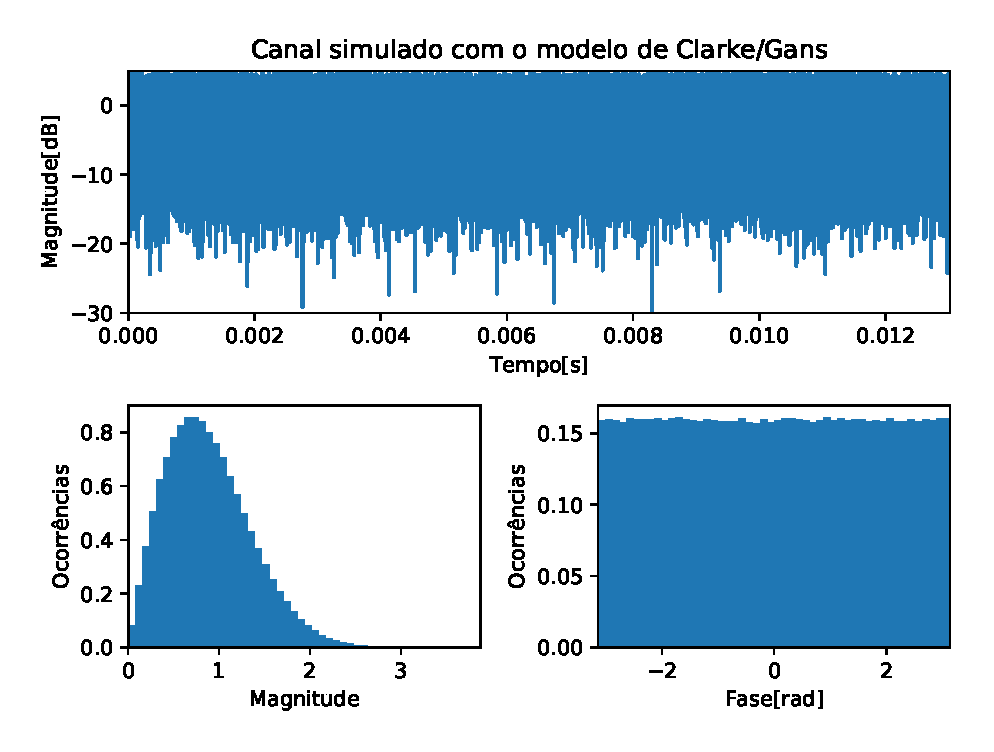
\includegraphics[scale=0.55]{gans_060kmh.eps}
    \caption{Canal simulado com o modelo de Clarke/Gans com uma velocidade relativa de 60km/h}
    \label{fig:gans-60km-h}
\end{figure}
\begin{figure}[h!]
    \centering
    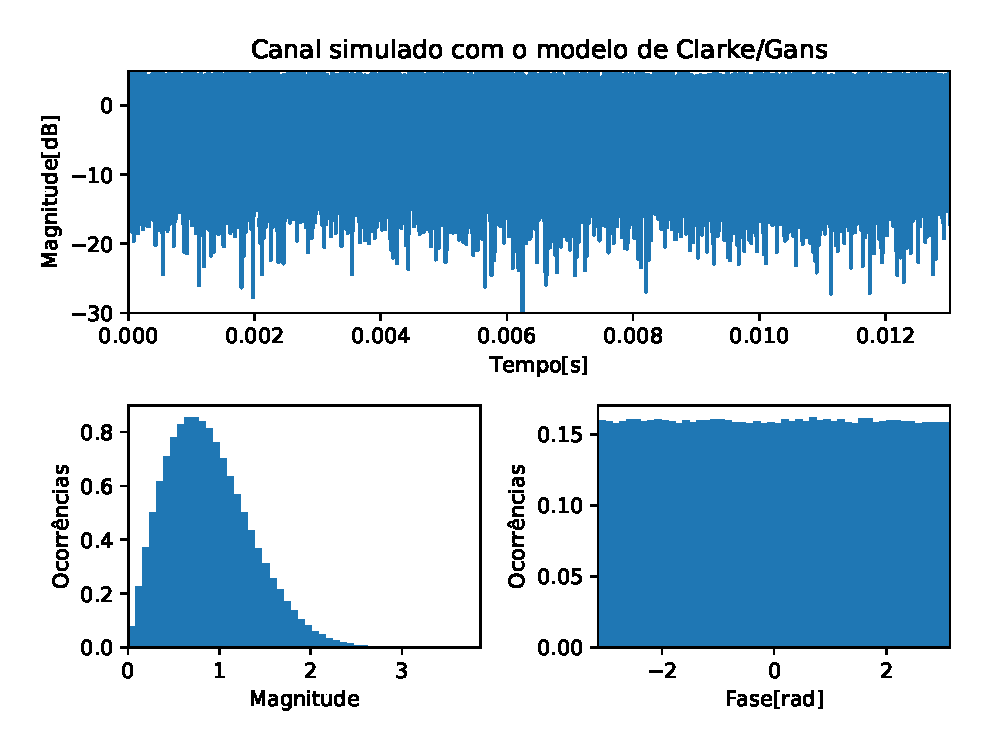
\includegraphics[scale=0.55]{gans_120kmh.eps}
    \caption{Canal simulado com o modelo de Clarke/Gans com uma velocidade relativa de 120km/h}
    \label{fig:gans-120km-h}
\end{figure}
\subsection{Modelo de Jakes}
Esse modelo foi proposto em \cite{jakes}. \cite{mimo} mostra que o modelo de Jakes, diferente do modelo de Clarke/Gans, parte da geração de múltiplas senóides complexas. Esse modelo foi inicialmente proposto com o foco em simulações em hardware, por passar a depender da geração de senóides (comumente tabeladas em hardware) ao invés da geração de números aleatórios a partir de uma variável aleatória específica.

\section{Conclusões}

Nas simulações que utilizaram o modelo de Clarke/Gans, percebe-se que, conforme é-se dito, em \cite{gans}, "a densidade de probabilidade da amplitude é Rayleigh enquanto a fase é uniformemnte distribuída", comportamentos claramente observáveis nos gráficos.

Para velocidades maiores, pudemos observar atenuações maiores causadas pelo canal comparando às velocidade relativa inferiores. Isso pode indicar  uma seletividade no tempo.

Durante o desenvolvimento desse trabalho, observou-se uma complexidade maior do que a primeira parte do trabalho. Nessa segunda etapa, foi-se necessária maior maturidade matemática e científica, dado que foi necessário analisar com maior atenção a respectiva referência. Além disso, o poder computacional disponível nos momentos reservados para a execução desse projeto não foram capazes de rodar as simulações em tempo hábil. Dessa forma, tem-se apenas os gráficos apresentados porque os demais não finalizaram seus respectivos cálculos.

Uma versão inicial do modelo de Jakes foi feita, embora ainda precise de correções. Continuarei trabalhando nesse projeto mesmo com o prazo para envio finalizado.

\bibliographystyle{IEEEtran}
\bibliography{some_books,some_urls}

\end{document}
